\documentclass{article}
\usepackage{geometry}
\geometry{a4paper, margin=1in}
\usepackage{amsmath}
\usepackage{graphicx}
\usepackage{hyperref}
\usepackage{booktabs}
% Make czech characters work
%  \usepackage[czech]{babel}
%add package for python code
\usepackage{listings}
\usepackage{color}
\usepackage{float}
\usepackage{subcaption}
\usepackage{tikz}
\usepackage{pgfplots}
\usepackage{pgfplotstable}
\usepackage{filecontents}
\usepackage{hyperref}
\usepackage{xcolor}
\usepackage{alltt}

\pgfplotsset{compat=1.18}

\lstset{
    language=Bash,
    basicstyle=\ttfamily\small,
    keywordstyle=\color{blue},
    stringstyle=\color{red},
    commentstyle=\color{green},
    showstringspaces=false,
    numbers=left,
    numberstyle=\tiny\color{gray},
    breaklines=true,
    frame=single,
    inputencoding=utf8
}

\title{Zápočet - výsledky}
\author{Tomáš Jelínek}
\date{\today}

\begin{document}

\maketitle
\tableofcontents

\section{Description of the assignment}
The following sequence was obtained during sequencing of an environmental sample off the coast
of Antarctica:

\begin{verbatim}
GAGTTTGATCCTGGCTCAGGATGAACGCTAGCGGCAGGCTTAACACATGCAAGTCGAGGGGTAACATTGTAG
CTTGCTACAGATGACGACCGGCGCACGGGTGCGTAACGCGTATACAATTTACCTATTACTAAGAGATAGCCCA
GAGAAATTTGGATTAATATTTTATAGCATTATCGATTGGCATCAATTGGTAATTAAAGATTACGGTAATAGATG
AGTATGCGTCCTATTAGCTTGATGGTAAGGTAACGGCTTACCATGGCTACGATAGGTAGGGGTCCTGAGAGG
GAGATCCACCACACTGGTACTGAGACACGGACCAGACTCCTACGGGAGGCAGCAGTGAGGAATATTGGACAA
TGGGAGCAATCCTGATCCAGCCATGCCGCGTGCAGGAAGACTGCCCTATGGGTTGTAAACTGCTTTTATACAG
GAAGAAAACGGTTCACGTGTGAACTGTTGACGGTACTGTAGGAATAAGGATCGGCTAACTCCGTGCCAGCAG
CCGCGGTAATACGGAGGATCCAGGCGTTATCCGGAATCATTGGGTTTAAAGGGTCCGTAGGCGGGACAATCA
GTCAGTGGTGAAAGTTTGCGGCTCAACCGTAAAATTGCCATTGATACTGTTGTTCTTGAGTGCTTGTGAAGTG
GTTAGAATGAGTAGTGTAGAAATGAAATGCATAGATATTACTCAGAATACCGATTGCGAAGGCAGATCACTA
ACAATTCACTGACGCTGATGGACGAAAGCGTAGTAGCGAACAGGATTAGATACCCTGGTAGTCTACGCCGTA
AACGATGGTTACTAGCTGTTCGGACTAATTGCGGTCTGAGTGGCTAAGCGAAAGTGATAAGTAACCCACCTG
GGGAGTACGTTCGCAAGAATGAAACTCAAAGGAATTGACGGGGGCCCGCACAAGCGGTGGAGCATGTGGTT
TAATATGATACGCGAGGAACCTTACCAGGGCTTAAATGCAGTTTGACAGGGGTGGAAACATCTTTTTCTTCGG
ACAAATTGCAAGGTGCTGCATGGTTGTCGTCAGCTCGTGCCGTGAGGTGTCAGGTTAAGTCCTTATAACGAGC
GCAACCCCTTTGTTTAGTTACCAGCATGTAAAGATGGGGACTCTAGACATACTGCCAGTGTAAACTGTGAGGA
AGGTGGGGATGACGTCAAATCATCACGGCCCTTACGTCCTGGGCTACACACGTGCTACAATGGTAGGGACAG
AGAGCAGCCACTGGGTGACCAGGAGCGAATCTACAAACCCTATCACAGTTCGGATCGCAGTCTGCAACTCGA
CTGCGTGAAGCTGGAATCGCTAGTAATATACAGCCATGATGCGGTGAATACGTTCCCGGGCCTTGTACACACC
GCCCGTCAAGCCATGGAAGCTGGGGGTACCTGAAGTCGGTCGCCGCAAGGAGCCGCCTAGGGTAAAACTAG
TAACTGGGGCTAAGTCGTAACAAGGTAACC
\end{verbatim}

Based on the sequence similarity, determine the function of this protein and which group of
organisms it comes from. Show this on a phylogenetic tree constructed by any method, which you
learned, that includes at least 50 homologues from the GenBank database. When you calculate the
tree, do not forget to calculate the branch support (bootstrap or posterior probability). Present the
tree in a way (rooting, labelling taxa, supports) that appropriately and clearly illustrates your
conclusions.

\section{Methods}

\subsection{Sequence similarity search}

I have inputed the sequence into the \url{https://web.expasy.org/translate/} tool to see the aminoacid sequence of the tanslated DNA sequence, however there were many stop codons (resulting into protein breaks) in all of the reading frames even for non common genetic codes (mitochondrials, hexaminita nuclears etc.).

This signifies that the sequence is not protein but rather something else. \textit{GAGTT} start is very common for 16s RNA sequences. This sequence was confirmed to be 16s RNA sequence by doing BLAST nucleotide search at NCBI.
\\
For the results of the search \ref{sec:first_blast} see the Appendix \ref{sec:appendix}.

\subsection{16s RNA sequence search}

Because the sequence is 16s RNA, I have used database of these seqs to search for homologues. I have made a new NCBI search where I have changed the database to \textit{16s ribosomal RNA sequences (Bacteria and Archaea)} and I have used the same sequence as a query.
\\
For the params and results of the search see \ref{sec:16s_blast} in the Appendix \ref{sec:appendix}.
\\
\\
Then from GeneBank I have downloaded the sequences of the first 100 hits (see \ref{sec:genebank_seqs}) for the tree construction.

\subsection{Multiple sequence alignment}

I have done the MSA using MAFFT tool. The command used was:
\begin{lstlisting}[language=Bash, basicstyle=\ttfamily\small, keywordstyle=\color{blue}, stringstyle=\color{red}, commentstyle=\color{green}, showstringspaces=false, numbers=left, numberstyle=\tiny\color{gray}, breaklines=true, frame=single, inputencoding=utf8]
mafft --auto --clustalout genbank16s.fasta >16s_rna_seqs.mafft.clw
\end{lstlisting}

\subsection{Phylogenetic tree construction}

I have uset \textit{IQ-TREE} tool to construct the tree. The command used was:

\begin{lstlisting}[language=Bash, basicstyle=\ttfamily\small, keywordstyle=\color{blue}, stringstyle=\color{red}, commentstyle=\color{green}, showstringspaces=false, numbers=left, numberstyle=\tiny\color{gray}, breaklines=true, frame=single, inputencoding=utf8]
    iqtree -s alignment_file.phy -m GTR+G+I -bb 1000 -nt AUTO
\end{lstlisting}

The computation was done on the MetaCentrum cluster.
\\
\\
Resulting tree was visualized using \textit{iTOL} tool and is provided bellow.

\section{Results}

\begin{figure}[H]
    \centering
    \includegraphics[width=0.8\textwidth]{figs/trees/fJdOTooIUdYrX-yxf8qbfA-cropped.pdf}
    \caption{Circular phylogenetic tree of the 16s RNA sequences homologues}
    \label{fig:circular_phylogenetic_tree}
\end{figure}


\subsection{Discussion of the results}
As shown per blast the closest homologues are from the \textit{Psychroflexus} genus, especialy being closest with \textit{Psychroflexus torquis} having a 98.76\% identity.

\subsubsection{Conclusion}
The sequence is not a protein but rather a 16s RNA sequence from the \textit{Psychroflexus} genus. With it most likely being from the \textit{Psychroflex torquis} species, however the sequence identity is less than 99\% and further investigation would be needed to confirm the species.

\begin{figure}[H]
    \centering
    \includegraphics[width=0.8\textwidth]{figs/trees/TgSrFzuybyON3sXrNRgv1Q.pdf}
    \caption{Phylogenetic tree of the 16s RNA sequences homologues}
    \label{fig:phylogenetic_tree}
\end{figure}

%%%%%%%% APPENDIX %%%%%%%%

\section{Appendix}
\label{sec:appendix}

\subsection{First BLAST search}
\label{sec:first_blast}
\begin{figure}[H]
    \centering
    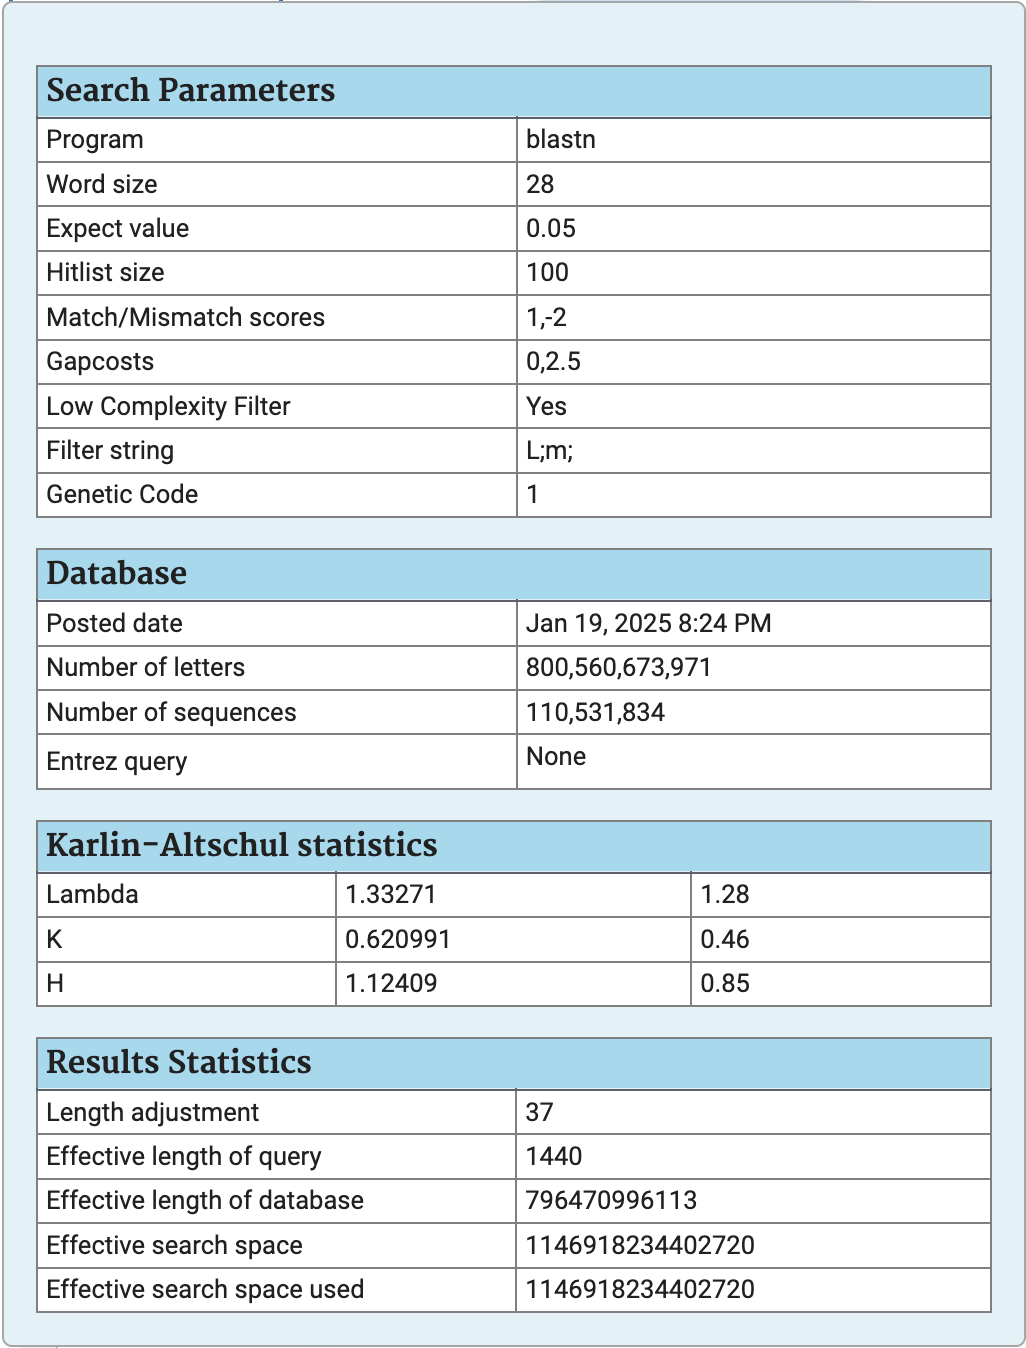
\includegraphics[width=0.8\textwidth]{figs/blast_all_seq_params.png}
    \caption{BLAST search parameters}
\end{figure}

\begin{figure}[H]
    \centering
    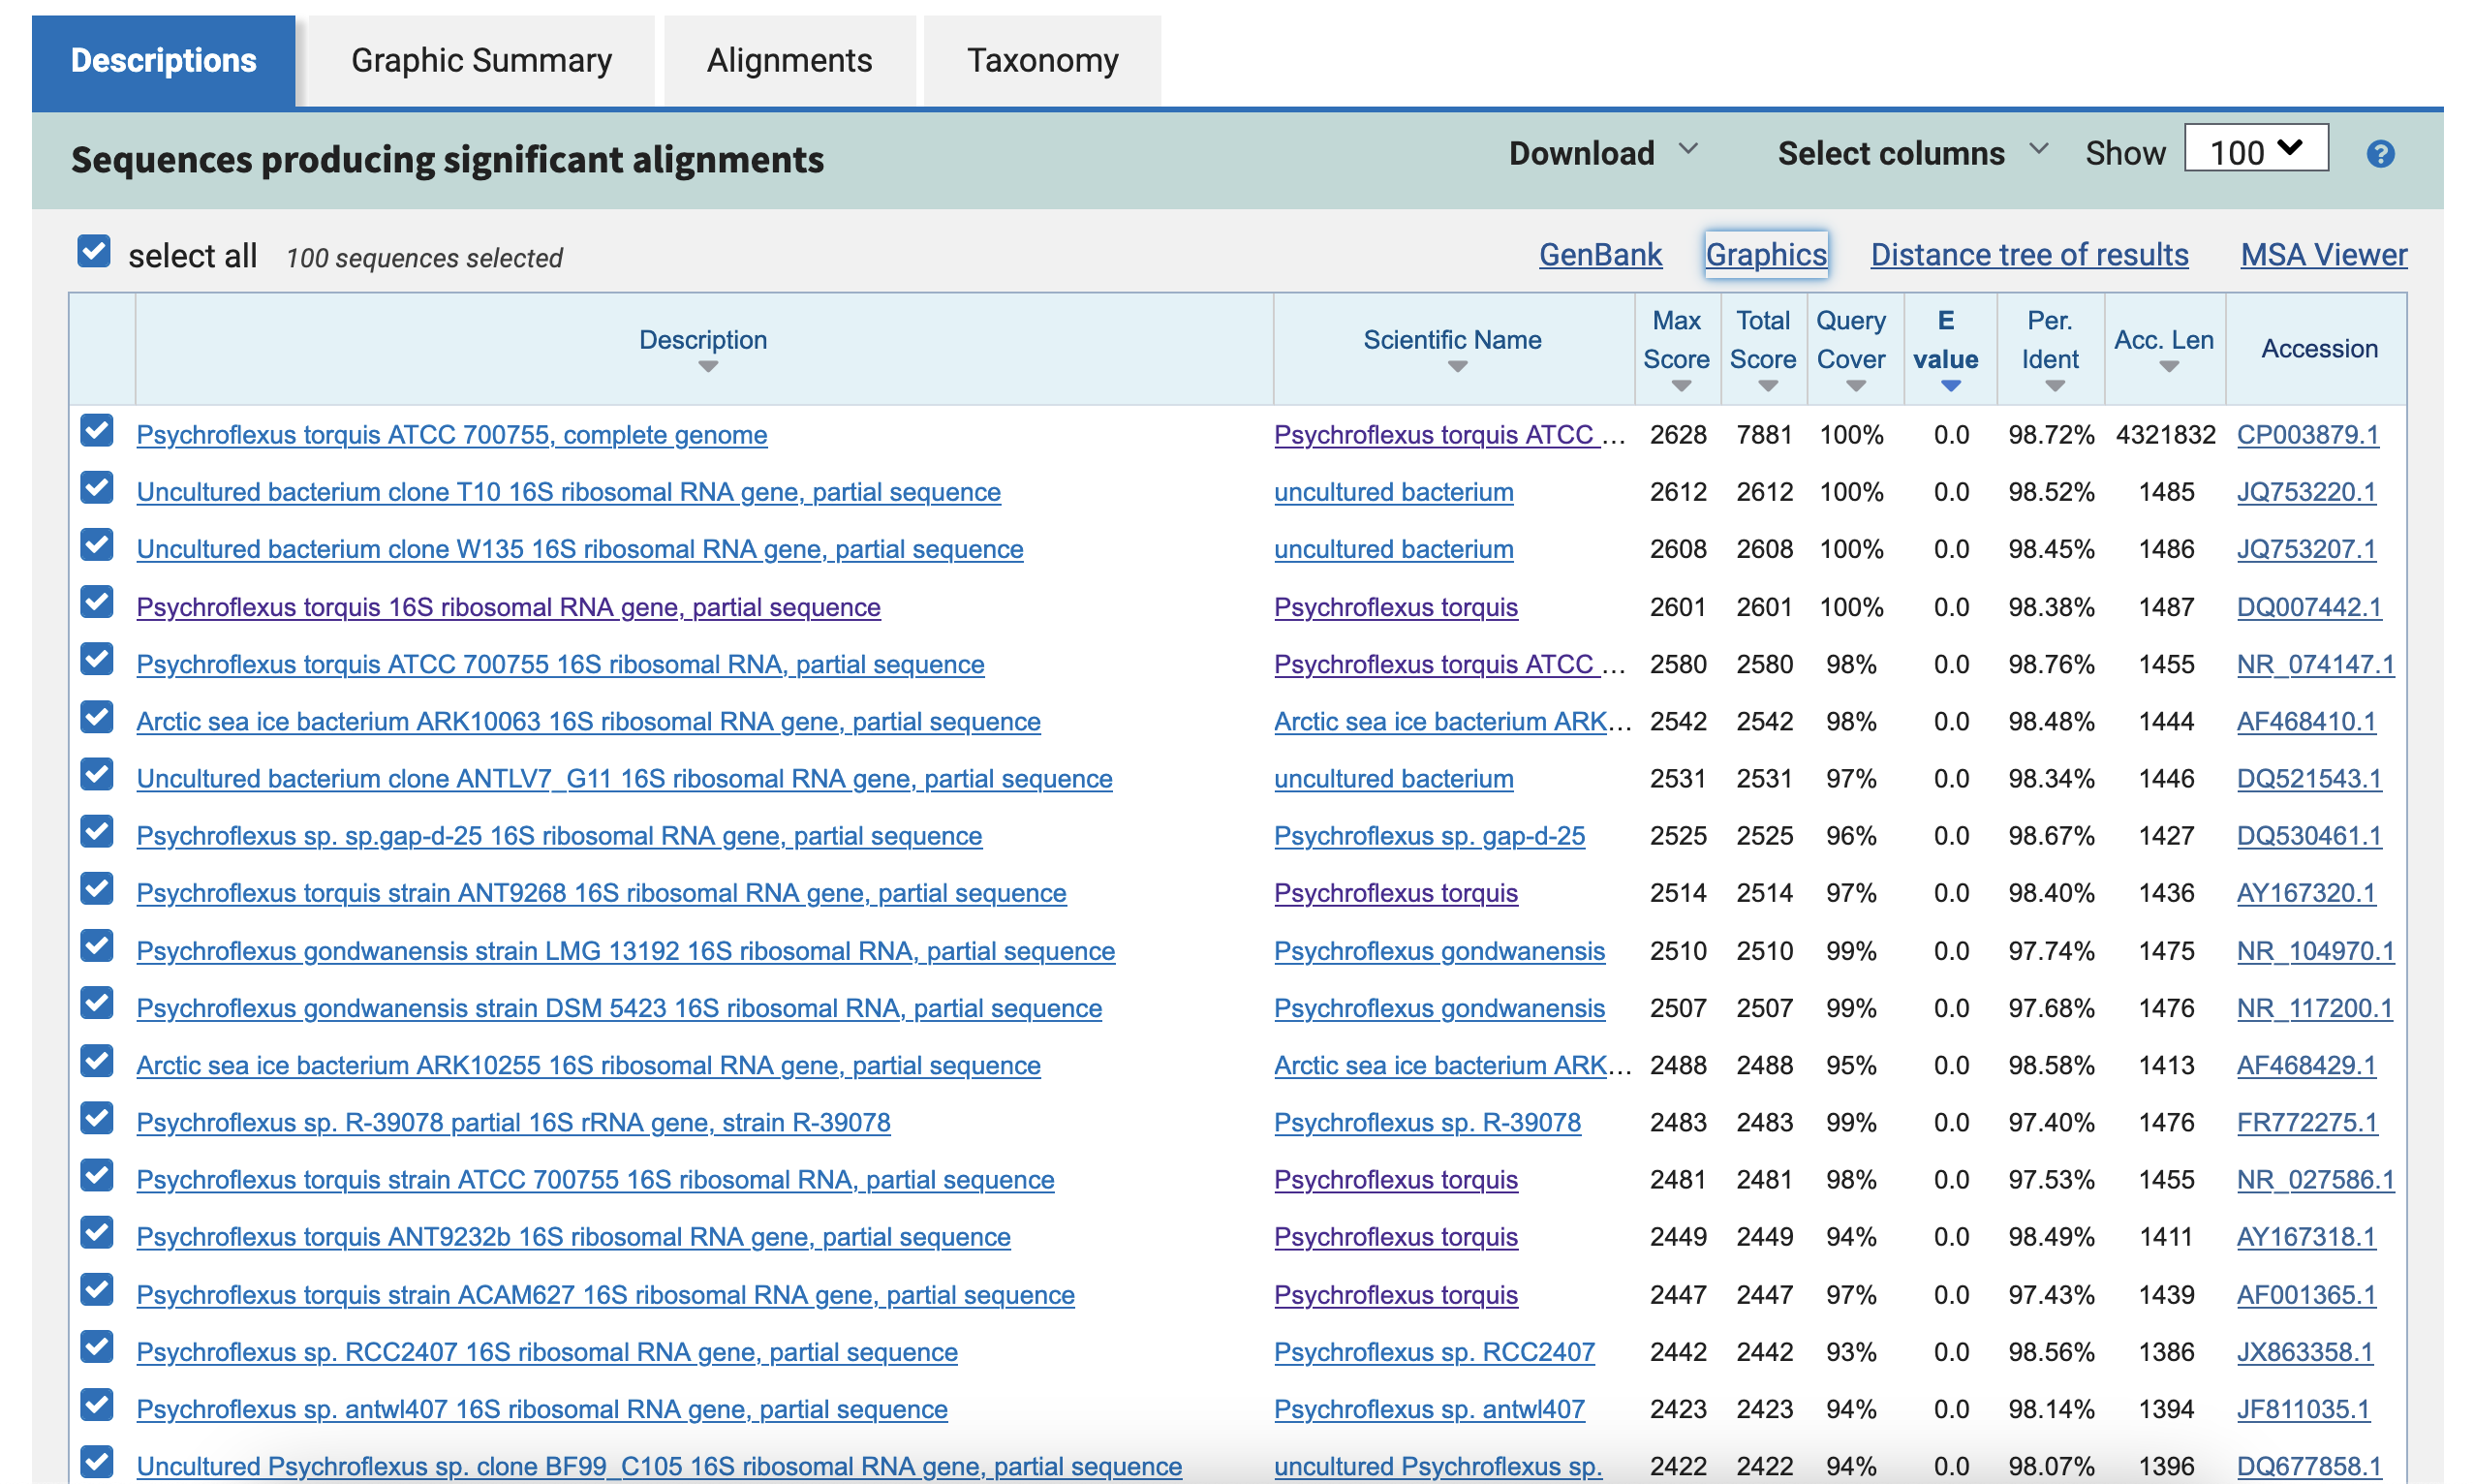
\includegraphics[width=0.95\textwidth]{figs/all_seq_search.png}
    \caption{BLAST search results}
\end{figure}

\subsection{16s RNA search database BLASTn seach}
\label{sec:16s_blast}

\begin{figure}[H]
    \centering
    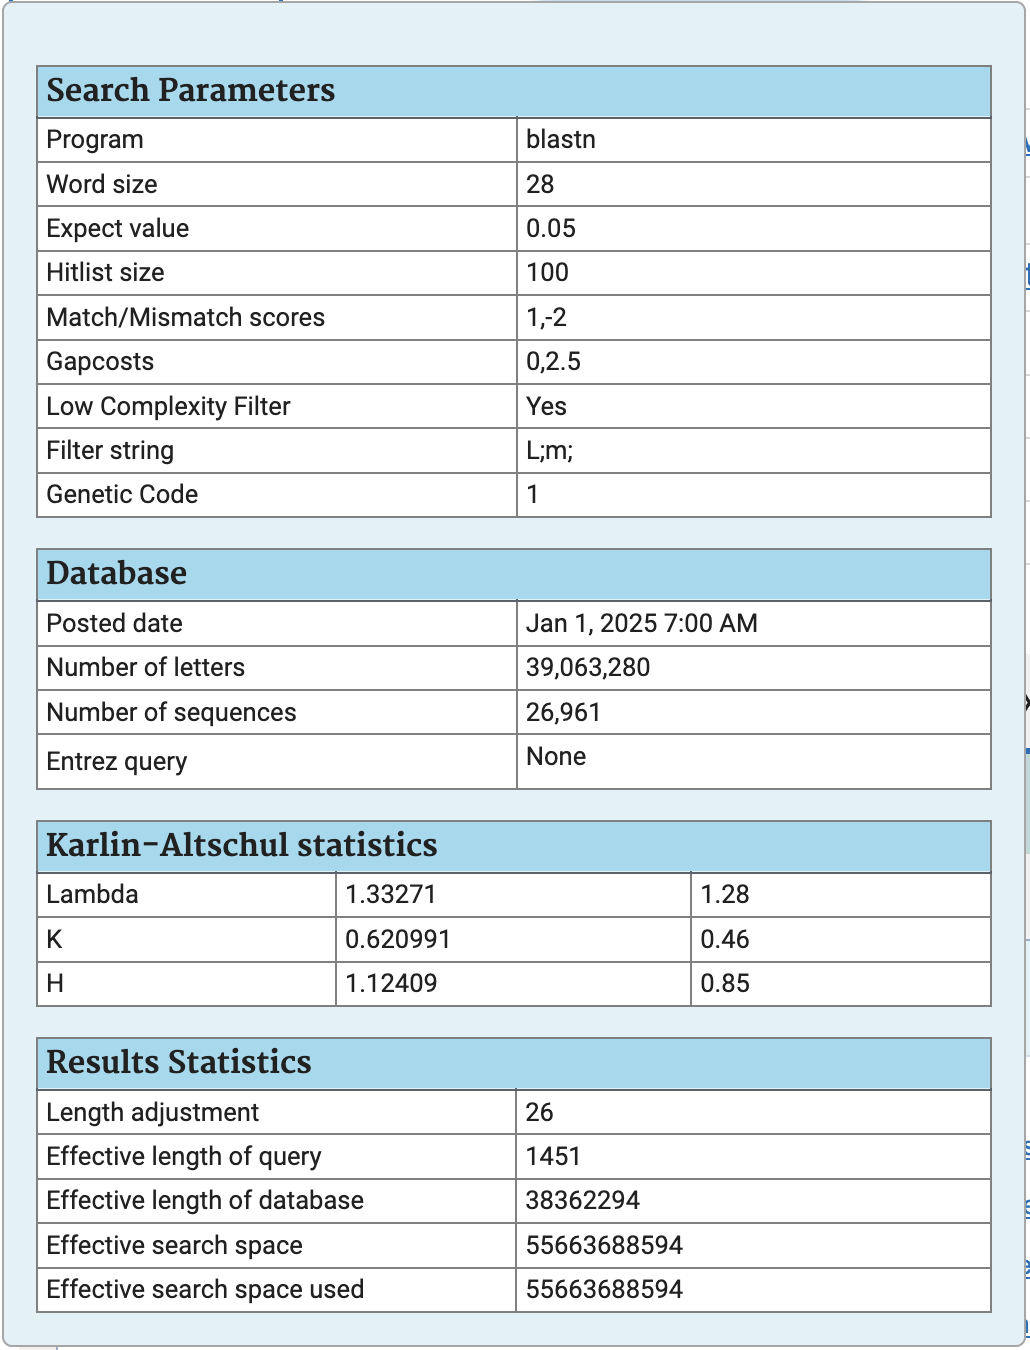
\includegraphics[width=0.8\textwidth]{figs/blast_16s_params.png}
    \caption{BLAST search parameters}
\end{figure}

\subsection{GeneBank downloaded sequences}
\label{sec:genebank_seqs}

\begin{figure}[H]
    \centering
    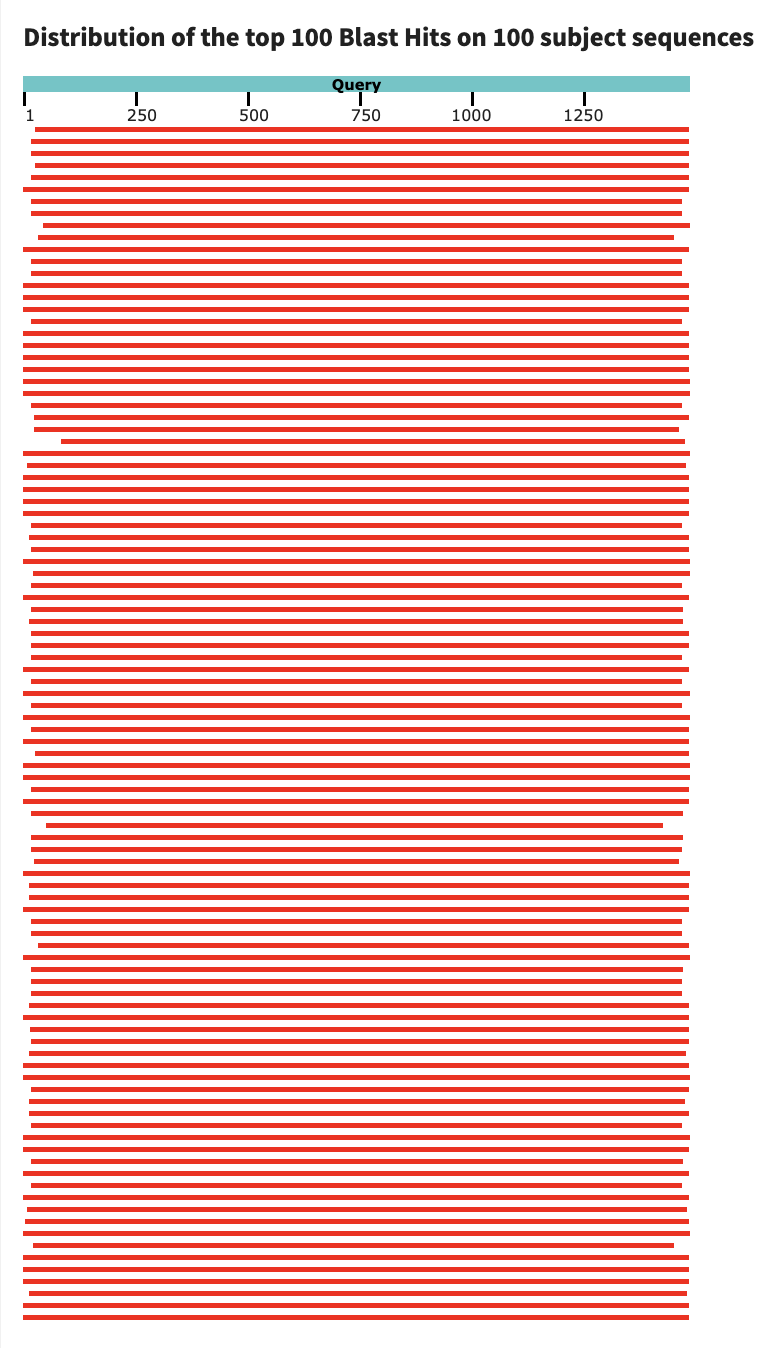
\includegraphics[width=0.8\textwidth]{figs/100_blast_seqs.png}
    \caption{First 100 sequences from the search}
\end{figure}

\begin{verbatim}
    1	>NR_074147.1 Psychroflexus torquis ATCC 700755 16S ribosomal RNA, partial sequence
    2	>NR_104970.1 Psychroflexus gondwanensis strain LMG 13192 16S ribosomal RNA, partial sequence
    3	>NR_117200.1 Psychroflexus gondwanensis strain DSM 5423 16S ribosomal RNA, partial sequence
    4	>NR_027586.1 Psychroflexus torquis strain ATCC 700755 16S ribosomal RNA, partial sequence
    5	>NR_044410.1 Psychroflexus sediminis strain YIM C238 16S ribosomal RNA, partial sequence
    6	>NR_180905.1 Psychroflexus aurantiacus strain YR1-1 16S ribosomal RNA, partial sequence
    7	>NR_108235.1 Psychroflexus salinarum strain ISL-14 16S ribosomal RNA, partial sequence
    8	>NR_149277.1 Psychroflexus aestuariivivens strain DB-3 16S ribosomal RNA, partial sequence
    9	>NR_112778.1 Psychroflexus lacisalsi strain H7 16S ribosomal RNA, partial sequence
   10	>NR_028854.1 Psychroflexus tropicus strain LA1 16S ribosomal RNA, partial sequence
   11	>NR_108506.1 Psychroflexus halocasei strain WCC 4520 16S ribosomal RNA, partial sequence
   12	>NR_153694.1 Psychroflexus saliphilus strain WDS4A13 16S ribosomal RNA, partial sequence
   13	>NR_147723.1 Psychroflexus salis strain X15M-6 16S ribosomal RNA, partial sequence
   14	>NR_180658.1 Antarcticibacterium arcticum strain PAMC 28998 16S ribosomal RNA, partial sequence
   15	>NR_043907.1 Salinimicrobium catena strain HY1 16S ribosomal RNA, partial sequence
   16	>NR_181138.1 Salinimicrobium oceani strain J15B91 16S ribosomal RNA, partial sequence
   17	>NR_147724.1 Psychroflexus planctonicus strain X15M-8 16S ribosomal RNA, partial sequence
   18	>NR_074656.1 Zunongwangia profunda SM-A87 strain SMA-87 16S ribosomal RNA, partial sequence
   19	>NR_116794.1 Aquimarina agarilytica ZC1 16S ribosomal RNA, partial sequence
   20	>NR_125622.1 Zunongwangia atlantica 22II14-10F7 16S ribosomal RNA, partial sequence
   21	>NR_136419.1 Aquimarina penaei strain P3-1 16S ribosomal RNA, partial sequence
   22	>NR_159278.1 Antarcticibacterium flavum strain JB01H24 16S ribosomal RNA, partial sequence
   23	>NR_151968.1 Aquimarina aggregata strain RZW4-3-2 16S ribosomal RNA, partial sequence
   24	>NR_109368.1 Salinimicrobium gaetbulicola strain BB-My20 16S ribosomal RNA, partial sequence
   25	>NR_044408.1 Salinimicrobium terrae strain YIM-C338 16S ribosomal RNA, partial sequence
   26	>NR_043758.1 Mesonia mobilis DSM 19841 strain KMM 6059 16S ribosomal RNA, partial sequence
   27	>NR_157716.1 Zunongwangia endophytica strain CPA58 16S ribosomal RNA, partial sequence
   28	>NR_126228.1 Salegentibacter echinorum strain HD4 16S ribosomal RNA, partial sequence
   29	>NR_126281.1 Zunongwangia mangrovi strain P2E16 16S ribosomal RNA, partial sequence
   30	>NR_181137.1 Salinimicrobium nanhaiense strain J15B81-2 16S ribosomal RNA, partial sequence
   31	>NR_180157.1 Constantimarinum furrinae strain ALE3EI 16S ribosomal RNA, complete sequence
   32	>NR_180113.1 Salegentibacter lacus strain LM13S 16S ribosomal RNA, partial sequence
   33	>NR_043986.1 Zunongwangia profunda SM-A87 strain SMA-87 16S ribosomal RNA, partial sequence
   34	>NR_180945.1 Psychroflexus maritimus strain C1 16S ribosomal RNA, partial sequence
   35	>NR_147777.1 Salinimicrobium soli strain CAU 1287 16S ribosomal RNA, partial sequence
   36	>NR_042444.1 Aquimarina intermedia strain R-28470 16S ribosomal RNA, partial sequence
   37	>NR_133696.1 Aquimarina pacifica strain SW150 16S ribosomal RNA, partial sequence
   38	>NR_043099.1 Salegentibacter flavus strain Fg 69 16S ribosomal RNA, partial sequence
   39	>NR_178995.1 Salegentibacter sediminis strain K5023 16S ribosomal RNA, partial sequence
   40	>NR_181555.1 Salegentibacter maritimus strain F63223 16S ribosomal RNA, partial sequence
   41	>NR_113917.1 Gillisia mitskevichiae strain NBRC 100590 16S ribosomal RNA, partial sequence
   42	>NR_115876.1 Sufflavibacter maritimus strain IMCC 1001 16S ribosomal RNA, partial sequence
   43	>NR_044244.1 Salegentibacter salarius strain ISL-6 16S ribosomal RNA, partial sequence
   44	>NR_042606.1 Algibacter mikhailovii strain LMG 23988 16S ribosomal RNA, partial sequence
   45	>NR_158098.1 Salinimicrobium flavum strain X7 16S ribosomal RNA, partial sequence
   46	>NR_148258.1 Aquimarina atlantica strain 22II-S11-z7 16S ribosomal RNA, partial sequence
   47	>NR_109623.1 Gillisia marina strain CBA3202 16S ribosomal RNA, partial sequence
   48	>NR_126240.1 Altibacter lentus strain JLT2010 16S ribosomal RNA, partial sequence
   49	>NR_117859.1 Aquimarina addita strain JC2680 16S ribosomal RNA, partial sequence
   50	>NR_136880.1 Pseudalgibacter alginicilyticus strain HZ22 16S ribosomal RNA, partial sequence
   51	>NR_117409.1 Salinimicrobium marinum strain KMM 6270 16S ribosomal RNA, partial sequence
   52	>NR_029076.1 Formosa algae strain F89 16S ribosomal RNA, partial sequence
   53	>NR_025944.1 Salegentibacter salegens strain DSM 5424 16S ribosomal RNA, partial sequence
   54	>NR_147717.1 Aquimarina hainanensis strain M124 16S ribosomal RNA, partial sequence
   55	>NR_125633.1 Christiangramia flava JLT2011 16S ribosomal RNA, partial sequence
   56	>NR_157624.1 Olleya algicola strain 3Alg 18 16S ribosomal RNA, partial sequence
   57	>NR_180546.1 Haloflavibacter putidus strain PLHSN227 16S ribosomal RNA, partial sequence
   58	>NR_113966.1 Nonlabens tegetincola strain NBRC 100970 16S ribosomal RNA, partial sequence
   59	>NR_134147.1 Psychroflexus salarius strain MIC1008 16S ribosomal RNA, partial sequence
   60	>NR_114005.1 Nonlabens tegetincola strain NBRC 101533 16S ribosomal RNA, partial sequence
   61	>NR_041300.1 Nonlabens tegetincola strain CKA-5 16S ribosomal RNA, partial sequence
   62	>NR_025822.1 Gillisia mitskevichiae strain KMM 6034 16S ribosomal RNA, partial sequence
   63	>NR_159216.1 Changchengzhania lutea strain SM1355 16S ribosomal RNA, partial sequence
   64	>NR_126191.1 Tamlana sedimentorum strain n6 16S ribosomal RNA, partial sequence
   65	>NR_133851.1 Salegentibacter chungangensis strain CAU 1289 16S ribosomal RNA, partial sequence
   66	>NR_102491.1 Nonlabens dokdonensis 16S ribosomal RNA, partial sequence
   67	>NR_145533.1 Algitalea ulvae strain 38-Ka-2 16S ribosomal RNA, partial sequence
   68	>NR_179123.1 Aquimarina celericrescens strain NS08 16S ribosomal RNA, partial sequence
   69	>NR_116100.1 Olleya marilimosa CAM030 16S ribosomal RNA, partial sequence
   70	>NR_159282.1 Christiangramia antarctica strain GDMCC 1.1208 16S ribosomal RNA, partial sequence
   71	>NR_113918.1 Salegentibacter mishustinae strain NBRC 100592 16S ribosomal RNA, partial sequence
   72	>NR_136817.1 Aquimarina agarivorans strain HQM9 16S ribosomal RNA, partial sequence
   73	>NR_165703.1 Zunongwangia flava strain MBLN094 16S ribosomal RNA, partial sequence
   74	>NR_156038.1 Nonlabens halophilus strain CAU 1131 16S ribosomal RNA, partial sequence
   75	>NR_109410.1 Christiangramia aestuarii strain BS12 16S ribosomal RNA, partial sequence
   76	>NR_043453.1 Psychroserpens mesophilus strain KOPRI 13649 16S ribosomal RNA, partial sequence
   77	>NR_042141.1 Gillisia limnaea DSM 15749 strain R-8282 16S ribosomal RNA, partial sequence
   78	>NR_157718.1 Mesonia maritima strain 15-S14-6 16S ribosomal RNA, partial sequence
   79	>NR_044376.1 Bizionia argentinensis JUB59 16S ribosomal RNA, partial sequence
   80	>NR_118560.1 Aquimarina megaterium XH134 16S ribosomal RNA, partial sequence
   81	>NR_043321.1 Aquimarina brevivitae strain SMK-19 16S ribosomal RNA, partial sequence
   82	>NR_044279.1 Ulvibacter antarcticus strain IMCC3101 16S ribosomal RNA, partial sequence
   83	>NR_148304.1 Tamlana nanhaiensis strain FHC16 16S ribosomal RNA, partial sequence
   84	>NR_109551.1 Olleya namhaensis strain WT-MY15 16S ribosomal RNA, partial sequence
   85	>NR_180661.1 Formosa maritima strain 1494 16S ribosomal RNA, partial sequence
   86	>NR_178920.1 Lacinutrix cladophorae strain 7Alg 4 16S ribosomal RNA, partial sequence
   87	>NR_113882.1 Salegentibacter holothuriorum strain NBRC 100249 16S ribosomal RNA, partial sequence
   88	>NR_181002.1 Aquimarina algicola strain M625 16S ribosomal RNA, partial sequence
   89	>NR_132290.1 Algibacter lectus strain WS-MY22 16S ribosomal RNA, partial sequence
   90	>NR_181090.1 Yeosuana marina strain JLT21 16S ribosomal RNA, complete sequence
   91	>NR_112971.1 Aquimarina macrocephali JAMB N27 16S ribosomal RNA, partial sequence
   92	>NR_104771.1 Nonlabens xylanidelens strain SW256 16S ribosomal RNA, partial sequence
   93	>NR_180792.1 Tamlana haliotis strain B1N29 16S ribosomal RNA, partial sequence
   94	>NR_042770.1 Formosa agariphila KMM 3901 16S ribosomal RNA, partial sequence
   95	>NR_145850.1 Formosa haliotis strain LMG 28520 16S ribosomal RNA, partial sequence
   96	>NR_135863.1 Algibacter psychrophilus strain PAMC 27237 16S ribosomal RNA, partial sequence
   97	>NR_179470.1 Winogradskyella vidalii strain HL634 16S ribosomal RNA, partial sequence
   98	>NR_159894.1 Aquimarina algiphila strain 9Alg 151 16S ribosomal RNA, partial sequence
   99	>NR_165774.1 Cellulophaga omnivescoria strain W5C 16S ribosomal RNA, complete sequence
  100	>NR_164965.1 Nonlabens xiamenensis strain 1Q3 16S ribosomal RNA, partial sequence
\end{verbatim}

\subsection{MAFFT log output}
\label{sec:mafft_log}
\begin{verbatim}
nthread = 0
nthreadpair = 0
nthreadtb = 0
ppenalty_ex = 0
stacksize: 8176 kb
generating a scoring matrix for nucleotide (dist=200) ... done
Gap Penalty = -1.53, +0.00, +0.00



Making a distance matrix ..

There are 51 ambiguous characters.
    1 / 100
done.

Constructing a UPGMA tree (efffree=0) ...
   90 / 100
done.

Progressive alignment 1/2...
STEP    74 / 99  f
Reallocating..done. *alloclen = 4053
STEP    99 / 99  f
done.

Making a distance matrix from msa..
    0 / 100
done.

Constructing a UPGMA tree (efffree=1) ...
   90 / 100
done.

Progressive alignment 2/2...
STEP    83 / 99  f
Reallocating..done. *alloclen = 4053
STEP    99 / 99  f
done.

disttbfast (nuc) Version 7.526
alg=A, model=DNA200 (2), 1.53 (4.59), -0.00 (-0.00), noshift, amax=0.0
0 thread(s)

distout=h
generating a scoring matrix for nucleotide (dist=200) ... done
dndpre (nuc) Version 7.526
alg=X, model=DNA200 (2), 1.53 (4.59), 0.37 (1.11), noshift, amax=0.0
0 thread(s)

minimumweight = 0.000010
autosubalignment = 0.000000
nthread = 0
randomseed = 0
blosum 62 / kimura 200
poffset = 0
niter = 2
sueff_global = 0.100000
nadd = 2
generating a scoring matrix for nucleotide (dist=200) ... done

   90 / 100
Segment   1/ 15    1-  54
STEP 002-058-1  identical.
Converged.

Segment   2/ 15   54- 144
Segment   3/ 15  142- 314.
STEP 002-012-1  identical.
Converged.

Segment   4/ 15  308- 421
STEP 002-098-1  identical.
Converged.

Segment   5/ 15  421- 553
STEP 002-098-1  identical.
Converged.

Segment   6/ 15  553- 704
STEP 002-013-1  identical.
Converged.

Segment   7/ 15  704- 809
STEP 002-078-1  identical.
Converged.

Segment   8/ 15  809- 929
STEP 002-098-1  rejected..
Converged.

Segment   9/ 15  929-1011
STEP 002-098-1  identical.
Converged.

Segment  10/ 15 1011-1020
STEP 002-098-1  identical.
Converged.

Segment  11/ 15 1020-1097
STEP 002-098-1  identical.
Converged.

Segment  12/ 15 1097-1248
STEP 002-098-1  identical.
Converged.

Segment  13/ 15 1248-1399
STEP 002-098-1  identical.
Converged.

Segment  14/ 15 1399-1482
STEP 002-035-1  identical.
Converged.

Segment  15/ 15 1482-1544
STEP 002-038-0  identical.
Converged.

done
dvtditr (nuc) Version 7.526
alg=A, model=DNA200 (2), 1.53 (4.59), -0.00 (-0.00), noshift, amax=0.0
0 thread(s)


Strategy:
 FFT-NS-i (Standard)
 Iterative refinement method (max. 2 iterations)

If unsure which option to use, try 'mafft --auto input > output'.
For more information, see 'mafft --help', 'mafft --man' and the mafft page.

The default gap scoring scheme has been changed in version 7.110 (2013 Oct).
It tends to insert more gaps into gap-rich regions than previous versions.
To disable this change, add the --leavegappyregion option.
\end{verbatim}

\subsection{IQ-TREE log output}

\begin{verbatim}
    IQ-TREE MPI multicore version 2.3.5.cmaple COVID-edition for Linux x86 64-bit built May 27 2024
    Developed by Bui Quang Minh, James Barbetti, Nguyen Lam Tung, Olga Chernomor,
    Heiko Schmidt, Dominik Schrempf, Michael Woodhams, Ly Trong Nhan, Thomas Wong
    
    Host:    cha.natur.cuni.cz (AVX512, FMA3, 187 GB RAM)
    Command: iqtree -s 16s_rna_seqs.mafft.clw -m GTR+G+I -bb 1000 -nt AUTO
    Seed:    561018 (Using SPRNG - Scalable Parallel Random Number Generator)
    Time:    Tue Jan 21 15:44:23 2025
    Kernel:  AVX+FMA - auto-detect threads (16 CPU cores detected)
    MPI:     1 processes
    
    Reading alignment file 16s_rna_seqs.mafft.clw ... Clustal format detected
    Alignment most likely contains DNA/RNA sequences
    Alignment has 100 sequences with 1544 columns, 539 distinct patterns
    379 parsimony-informative, 80 singleton sites, 1085 constant sites
                 Gap/Ambiguity  Composition  p-value
    Analyzing sequences: done in 0.000257905 secs using 99.26% CPU
       1  NR_074147.1    5.76%    passed     90.46%
       2  NR_104970.1    4.53%    passed     99.61%
       3  NR_117200.1    4.53%    passed     99.61%
       4  NR_027586.1    5.76%    passed     82.65%
       5  NR_044410.1    4.47%    passed     99.93%
       6  NR_180905.1    4.27%    passed     99.52%
       7  NR_108235.1    6.35%    passed    100.00%
       8  NR_149277.1    6.48%    passed     99.66%
       9  NR_112778.1    6.02%    passed     91.29%
      10  NR_028854.1    8.16%    passed     99.83%
      11  NR_108506.1    4.34%    passed     79.50%
      12  NR_153694.1    6.09%    passed     86.04%
      13  NR_147723.1    6.35%    passed     79.30%
      14  NR_180658.1    3.56%    passed     99.63%
      15  NR_043907.1    3.69%    passed     98.29%
      16  NR_181138.1    2.20%    passed     75.53%
      17  NR_147724.1    6.22%    passed     76.30%
      18  NR_074656.1    1.36%    passed     84.71%
      19  NR_116794.1    4.02%    passed     58.78%
      20  NR_125622.1    3.50%    passed     99.26%
      21  NR_136419.1    3.30%    passed     79.71%
      22  NR_159278.1    3.95%    passed     99.54%
      23  NR_151968.1    3.95%    passed     83.13%
      24  NR_109368.1    6.22%    passed     85.32%
      25  NR_044408.1    5.12%    passed     61.32%
      26  NR_043758.1    7.19%    passed     98.96%
      27  NR_157716.1    7.45%    passed     98.05%
      28  NR_126228.1    3.17%    passed     95.14%
      29  NR_126281.1    4.79%    passed     91.49%
      30  NR_181137.1    2.14%    passed     50.00%
      31  NR_180157.1    1.68%    passed     92.71%
      32  NR_180113.1    3.24%    passed     69.46%
      33  NR_043986.1    3.30%    passed     88.10%
      34  NR_180945.1    6.22%    passed     83.49%
      35  NR_147777.1    1.88%    passed     73.81%
      36  NR_042444.1    4.40%    passed     99.93%
      37  NR_133696.1    3.95%    passed     76.38%
      38  NR_043099.1    4.73%    passed     94.88%
      39  NR_178995.1    6.09%    passed     91.83%
      40  NR_181555.1    1.68%    passed     81.57%
      41  NR_113917.1    6.41%    passed     95.86%
      42  NR_115876.1    5.51%    passed     84.51%
      43  NR_044244.1    3.82%    passed     84.05%
      44  NR_042606.1    4.99%    passed     89.83%
      45  NR_158098.1    6.22%    passed     89.20%
      46  NR_148258.1    3.76%    passed     88.62%
      47  NR_109623.1    6.67%    passed     91.54%
      48  NR_126240.1    3.82%    passed     91.14%
      49  NR_117859.1    6.48%    passed     74.65%
      50  NR_136880.1    4.21%    passed     99.37%
      51  NR_117409.1    4.60%    passed     44.33%
      52  NR_029076.1    2.01%    passed     89.79%
      53  NR_025944.1    5.05%    passed     85.41%
      54  NR_147717.1    3.63%    passed     52.50%
      55  NR_125633.1    3.37%    passed     86.18%
      56  NR_157624.1    4.79%    passed     96.73%
      57  NR_180546.1    3.76%    passed     90.40%
      58  NR_113966.1    6.02%    passed     98.25%
      59  NR_134147.1   10.69%    passed     72.82%
      60  NR_114005.1    6.09%    passed     98.87%
      61  NR_041300.1    6.22%    passed     98.93%
      62  NR_025822.1    7.38%    passed     94.47%
      63  NR_159216.1    4.08%    passed     99.07%
      64  NR_126191.1    3.50%    passed     98.24%
      65  NR_133851.1    1.62%    passed     82.71%
      66  NR_102491.1    1.94%    passed     99.11%
      67  NR_145533.1    6.48%    passed     80.14%
      68  NR_179123.1    6.28%    passed     97.30%
      69  NR_116100.1    5.57%    passed     99.68%
      70  NR_159282.1    3.11%    passed     99.45%
      71  NR_113918.1    5.76%    passed     83.82%
      72  NR_136817.1    6.48%    passed     78.01%
      73  NR_165703.1    6.22%    passed     89.04%
      74  NR_156038.1    2.59%    passed     67.50%
      75  NR_109410.1    3.37%    passed     88.45%
      76  NR_043453.1    2.78%    passed     81.09%
      77  NR_042141.1    4.40%    passed     94.10%
      78  NR_157718.1    5.12%    passed     88.64%
      79  NR_044376.1    1.62%    passed     94.44%
      80  NR_118560.1    3.82%    passed     91.40%
      81  NR_043321.1    4.15%    passed     98.31%
      82  NR_044279.1    5.38%    passed     98.92%
      83  NR_148304.1    3.95%    passed     82.98%
      84  NR_109551.1    6.67%    passed     96.55%
      85  NR_180661.1    3.69%    passed     71.56%
      86  NR_178920.1    4.27%    passed     81.09%
      87  NR_113882.1    5.76%    passed     90.38%
      88  NR_181002.1    3.63%    passed     92.18%
      89  NR_132290.1    6.54%    passed     82.80%
      90  NR_181090.1    1.81%    passed     97.02%
      91  NR_112971.1    4.99%    passed     94.39%
      92  NR_104771.1    2.01%    passed     99.09%
      93  NR_180792.1    3.89%    passed     94.37%
      94  NR_042770.1    7.45%    passed     84.10%
      95  NR_145850.1    4.66%    passed     76.49%
      96  NR_135863.1    2.20%    passed     93.66%
      97  NR_179470.1    1.68%    passed     81.76%
      98  NR_159894.1    4.92%    passed     96.13%
      99  NR_165774.1    1.55%    passed     89.73%
     100  NR_164965.1    1.94%    passed     18.54%
    ****  TOTAL          4.53%  0 sequences failed composition chi2 test (p-value<5%; df=3)
    
    Create initial parsimony tree by phylogenetic likelihood library (PLL)... 0.102 seconds
    Generating 1000 samples for ultrafast bootstrap (seed: 561018)...
    
    NOTE: 9 MB RAM (0 GB) is required!
    Measuring multi-threading efficiency up to 16 CPU cores
    Increase to 10 rounds for branch lengths
    132 trees examined
    Threads: 1 / Time: 16.035 sec / Speedup: 1.000 / Efficiency: 100% / LogL: -31161
    Threads: 2 / Time: 12.965 sec / Speedup: 1.237 / Efficiency: 62% / LogL: -31161
    Threads: 3 / Time: 9.883 sec / Speedup: 1.622 / Efficiency: 54% / LogL: -31161
    Threads: 4 / Time: 10.513 sec / Speedup: 1.525 / Efficiency: 38% / LogL: -31161
    BEST NUMBER OF THREADS: 3
    
    Estimate model parameters (epsilon = 0.100)
    Thoroughly optimizing +I+G parameters from 10 start values...
    Init pinv, alpha: 0.000, 1.000 / Estimate: 0.000, 0.204 / LogL: -19708.070
    Init pinv, alpha: 0.078, 1.000 / Estimate: 0.665, 0.727 / LogL: -19354.793
    Init pinv, alpha: 0.156, 1.000 / Estimate: 0.665, 0.725 / LogL: -19354.797
    Init pinv, alpha: 0.234, 1.000 / Estimate: 0.665, 0.727 / LogL: -19354.786
    Init pinv, alpha: 0.312, 1.000 / Estimate: 0.665, 0.725 / LogL: -19354.799
    Init pinv, alpha: 0.390, 1.000 / Estimate: 0.665, 0.726 / LogL: -19354.800
    Init pinv, alpha: 0.468, 1.000 / Estimate: 0.665, 0.726 / LogL: -19354.800
    Init pinv, alpha: 0.547, 1.000 / Estimate: 0.665, 0.725 / LogL: -19354.808
    Init pinv, alpha: 0.625, 1.000 / Estimate: 0.665, 0.726 / LogL: -19354.799
    Init pinv, alpha: 0.703, 1.000 / Estimate: 0.666, 0.734 / LogL: -19354.782
    Optimal pinv,alpha: 0.666, 0.734 / LogL: -19354.782
    
    Parameters optimization took 4.177 sec
    Wrote distance file to... 
    Computing ML distances based on estimated model parameters...
    Calculating distance matrix: done in 0.0284079 secs using 309.3% CPU
    Computing ML distances took 0.028610 sec (of wall-clock time) 0.088075 sec (of CPU time)
    Setting up auxiliary I and S matrices: done in 0.000436875 secs using 284.1% CPU
    Computing RapidNJ tree took 0.019404 sec (of wall-clock time) 0.035566 sec (of CPU time)
    Log-likelihood of RapidNJ tree: -19448.421
    --------------------------------------------------------------------
    |             INITIALIZING CANDIDATE TREE SET                      |
    --------------------------------------------------------------------
    Generating 98 parsimony trees... 1.406 second
    Computing log-likelihood of 98 initial trees ... 1.003 seconds
    Current best score: -19329.248
    
    Do NNI search on 20 best initial trees
    Estimate model parameters (epsilon = 0.100)
    BETTER TREE FOUND at iteration 1: -19242.142
    Iteration 10 / LogL: -19340.074 / Time: 0h:0m:58s
    Iteration 20 / LogL: -19251.268 / Time: 0h:1m:0s
    Finish initializing candidate tree set (18)
    Current best tree score: -19242.142 / CPU time: 6.181
    Number of iterations: 20
    --------------------------------------------------------------------
    |               OPTIMIZING CANDIDATE TREE SET                      |
    --------------------------------------------------------------------
    Estimate model parameters (epsilon = 0.100)
    BETTER TREE FOUND at iteration 21: -19240.772
    Estimate model parameters (epsilon = 0.100)
    BETTER TREE FOUND at iteration 24: -19239.643
    Iteration 30 / LogL: -19241.215 / Time: 0h:1m:3s (0h:3m:22s left)
    Iteration 40 / LogL: -19241.701 / Time: 0h:1m:5s (0h:2m:19s left)
    Iteration 50 / LogL: -19242.724 / Time: 0h:1m:7s (0h:1m:40s left)
    Log-likelihood cutoff on original alignment: -19364.838
    Iteration 60 / LogL: -19242.330 / Time: 0h:1m:10s (0h:1m:15s left)
    Iteration 70 / LogL: -19249.683 / Time: 0h:1m:12s (0h:0m:56s left)
    Iteration 80 / LogL: -19242.476 / Time: 0h:1m:14s (0h:0m:41s left)
    Iteration 90 / LogL: -19239.709 / Time: 0h:1m:16s (0h:0m:29s left)
    Iteration 100 / LogL: -19240.679 / Time: 0h:1m:19s (0h:0m:19s left)
    Log-likelihood cutoff on original alignment: -19361.211
    NOTE: Bootstrap correlation coefficient of split occurrence frequencies: 0.998
    Iteration 110 / LogL: -19239.667 / Time: 0h:1m:21s (0h:1m:7s left)
    Iteration 120 / LogL: -19275.538 / Time: 0h:1m:24s (0h:0m:56s left)
    Total number of trees received: 0
    Total number of trees sent: 0
    Total number of NNI searches done by myself: 125
    TREE SEARCH COMPLETED AFTER 125 ITERATIONS / Time: 0h:1m:25s
    
    --------------------------------------------------------------------
    |                    FINALIZING TREE SEARCH                        |
    --------------------------------------------------------------------
    Performs final model parameters optimization
    Estimate model parameters (epsilon = 0.010)
    1. Initial log-likelihood: -19239.643
    Optimal log-likelihood: -19239.642
    Rate parameters:  A-C: 0.93221  A-G: 2.92346  A-T: 2.18332  C-G: 0.92367  C-T: 4.05160  G-T: 1.00000
    Base frequencies:  A: 0.273  C: 0.212  G: 0.289  T: 0.226
    Proportion of invariable sites: 0.664
    Gamma shape alpha: 0.681
    Parameters optimization took 1 rounds (0.028 sec)
    BEST SCORE FOUND : -19239.642
    Creating bootstrap support values...
    Split supports printed to NEXUS file 16s_rna_seqs.mafft.clw.splits.nex
    Total tree length: 4.249
    
    Total number of iterations: 125
    CPU time used for tree search: 86.631 sec (0h:1m:26s)
    Wall-clock time used for tree search: 30.755 sec (0h:0m:30s)
    Total CPU time used: 212.212 sec (0h:3m:32s)
    Total wall-clock time used: 85.447 sec (0h:1m:25s)
    
    Computing bootstrap consensus tree...
    Reading input file 16s_rna_seqs.mafft.clw.splits.nex...
    100 taxa and 485 splits.
    Consensus tree written to 16s_rna_seqs.mafft.clw.contree
    Reading input trees file 16s_rna_seqs.mafft.clw.contree
    Log-likelihood of consensus tree: -19240.812
    
    Analysis results written to: 
      IQ-TREE report:                16s_rna_seqs.mafft.clw.iqtree
      Maximum-likelihood tree:       16s_rna_seqs.mafft.clw.treefile
      Likelihood distances:          16s_rna_seqs.mafft.clw.mldist
    
    Ultrafast bootstrap approximation results written to:
      Split support values:          16s_rna_seqs.mafft.clw.splits.nex
      Consensus tree:                16s_rna_seqs.mafft.clw.contree
      Screen log file:               16s_rna_seqs.mafft.clw.log
    
    Date and Time: Tue Jan 21 15:45:49 2025
        
\end{verbatim}

\end{document}
